\section{Resolution of the Motivating Underestimation Example}
\label{sec:results-motivating-example}

Research Question~\ref{rq:motivating_example} examines whether FELICS resolves the underestimation identified by Matton et al.~\cite{mattonWalkTalkMeasuring2024} for MedQA question 521. To isolate the effect of joint interventions from stochastic concept extraction, the experiment uses exactly the nine concepts and current values reported by Matton et al.~\cite{mattonWalkTalkMeasuring2024} in their Table~9. The oracle places the patient's eating disorder, refusal of further treatment, and self-perception of weight in one candidate interaction group, and places the vital signs and treatment administered by EMS in a second group. The remaining four concepts form singleton groups.

The final consensus graph underlying this partition is shown in
Figure~\ref{fig:rq5-oracle-grouping}, and its retained pairwise co-grouping
frequencies are reported in Table~\ref{tab:rq5-cogrouping} in
Appendix~\ref{app:rq5-oracle-partition}.

Table~\ref{tab:hyp5-concept-ce-comparison} compares the causal effects reported by Matton et al.~\cite{mattonWalkTalkMeasuring2024} with the effects obtained in the controlled FELICS experiment. For the two newly evaluated models, the atomic and joint columns use the paired CE constructions defined in Section~\ref{sec:controlled_atomic_baseline}. The shift is defined as $\Delta\mathrm{CE}=\mathrm{CE}_{\mathrm{joint}}-\mathrm{CE}_{\mathrm{atomic}}$; positive values therefore indicate that FELICS credits a concept with a larger effect after accounting for its candidate interaction group.

\begin{table}[p]
  \centering
  \caption[Published and interaction-aware causal effects for the motivating MedQA example]{Causal effects for the nine concepts in the motivating MedQA example. The blue columns reproduce the singleton-intervention values reported by Matton et al.~\cite{mattonWalkTalkMeasuring2024}; the green columns contain the controlled experiment conducted in this work. Values from Matton et al.~\cite{mattonWalkTalkMeasuring2024} are available only to the two-decimal precision published in their Table~9.}
  \label{tab:hyp5-concept-ce-comparison}
  \resizebox{\textwidth}{!}{%
    \setlength{\tabcolsep}{3.4pt}%
    \renewcommand{\arraystretch}{1.12}%
    \pgfplotstabletypeset[
      col sep=comma,
      trim cells=true,
      columns={concept,matton_gpt35,matton_gpt4o,matton_claude,gpt_atomic,gpt_joint,gpt_delta,mistral_atomic,mistral_joint,mistral_delta},
      columns/concept/.style={column name={\textbf{Concept}},string type,column type=l},
      columns/matton_gpt35/.style={column name={\textbf{GPT-3.5}},column type={>{\columncolor{RoyalBlue!10}}r},fixed,fixed zerofill,precision=2},
      columns/matton_gpt4o/.style={column name={\textbf{GPT-4o}},column type={>{\columncolor{RoyalBlue!10}}r},fixed,fixed zerofill,precision=2},
      columns/matton_claude/.style={column name={\textbf{Claude}},column type={>{\columncolor{RoyalBlue!10}}r},fixed,fixed zerofill,precision=2},
      columns/gpt_atomic/.style={column name={\textbf{Atomic}},column type={>{\columncolor{ForestGreen!9}}r},fixed,fixed zerofill,precision=3},
      columns/gpt_joint/.style={column name={\textbf{Joint}},column type={>{\columncolor{ForestGreen!9}}r},fixed,fixed zerofill,precision=3},
      columns/gpt_delta/.style={column name={\textbf{$\Delta$CE}},column type={>{\columncolor{ForestGreen!9}}r},fixed,fixed zerofill,precision=3},
      columns/mistral_atomic/.style={column name={\textbf{Atomic}},column type={>{\columncolor{ForestGreen!9}}r},fixed,fixed zerofill,precision=3},
      columns/mistral_joint/.style={column name={\textbf{Joint}},column type={>{\columncolor{ForestGreen!9}}r},fixed,fixed zerofill,precision=3},
      columns/mistral_delta/.style={column name={\textbf{$\Delta$CE}},column type={>{\columncolor{ForestGreen!9}}r},fixed,fixed zerofill,precision=3},
      every head row/.style={before row={
        \hline
        & \multicolumn{3}{c}{\cellcolor{RoyalBlue!18}\textbf{Matton et al.~\cite{mattonWalkTalkMeasuring2024}}} &
        \multicolumn{3}{c}{\cellcolor{ForestGreen!16}\textbf{GPT-OSS 120B}} &
        \multicolumn{3}{c}{\cellcolor{ForestGreen!16}\textbf{Mistral Medium 3.5}}\\
      },after row=\hline},
      every last row/.style={after row=\hline},
    ]{data/rq5/concept_ce_comparison.csv}%
  }
\end{table}

The interaction-aware estimate increases the credited causal effect of the eating-disorder concept for both evaluated models: from $0.018$ to $0.029$ for GPT-OSS 120B and from $0.129$ to $0.145$ for Mistral Medium 3.5. This is consistent with the direction predicted in \rqref{rq:motivating_example}. The corresponding result for self-perception of weight, however, moves in the opposite direction, decreasing from $0.021$ to $0.017$ for GPT-OSS 120B and from $0.181$ to $0.033$ for Mistral Medium 3.5. The hypothesis requires the corrected estimate to increase for both motivating concepts and across all evaluated models. It is therefore only partially supported and cannot be accepted as stated.

\definecolor{HypFiveOne}{HTML}{1B9E77}
\definecolor{HypFiveTwo}{HTML}{D95F02}
\definecolor{HypFiveThree}{HTML}{7570B3}
\definecolor{HypFiveFour}{HTML}{E7298A}
\definecolor{HypFiveFive}{HTML}{66A61E}
\definecolor{HypFiveSix}{HTML}{E6AB02}
\definecolor{HypFiveSeven}{HTML}{A6761D}
\definecolor{HypFiveEight}{HTML}{1F78B4}
\definecolor{HypFiveNine}{HTML}{6A3D9A}

\newcommand{\HypFivePoint}[4]{%
  \addplot[only marks,mark=*,mark size=2.5pt,draw=#2,fill=#2]
    table[col sep=comma,x=#3,y=#4,
      restrict expr to domain={\thisrow{concept_id}}{#1:#1}]
    {data/rq5/concept_ce_identity.csv};%
}

% #1 title, #2 atomic column, #3 joint column, #4 upper axis limit.
\newcommand{\HypFiveIdentityPlot}[4]{%
  \begin{minipage}[t]{0.47\textwidth}
    \centering
    {\small\bfseries #1\par}
    \vspace{0.1em}
    \begin{tikzpicture}
      \begin{axis}[
        width=5.55cm,height=5.55cm,scale only axis,
        xmin=0,xmax=#4,ymin=0,ymax=#4,
        scaled ticks=false,
        xlabel={$\mathrm{CE}_{\mathrm{atomic}}$},
        ylabel={$\mathrm{CE}_{\mathrm{joint}}$},
        tick label style={font=\scriptsize,/pgf/number format/fixed,/pgf/number format/precision=2},
        label style={font=\scriptsize},
        grid=major,grid style={gray!18},axis line style={gray!60},
      ]
        \addplot[ResultScatterLine,very thick,dashed,domain=0:#4,samples=2] {x};
        \HypFivePoint{1}{HypFiveOne}{#2}{#3}
        \HypFivePoint{2}{HypFiveTwo}{#2}{#3}
        \HypFivePoint{3}{HypFiveThree}{#2}{#3}
        \HypFivePoint{4}{HypFiveFour}{#2}{#3}
        \HypFivePoint{5}{HypFiveFive}{#2}{#3}
        \HypFivePoint{6}{HypFiveSix}{#2}{#3}
        \HypFivePoint{7}{HypFiveSeven}{#2}{#3}
        \HypFivePoint{8}{HypFiveEight}{#2}{#3}
        \HypFivePoint{9}{HypFiveNine}{#2}{#3}
      \end{axis}
    \end{tikzpicture}
  \end{minipage}%
}

\begin{figure}[p]
  \centering
  \HypFiveIdentityPlot{GPT-OSS 120B}{gpt_atomic}{gpt_joint}{0.05}
  \hfill
  \HypFiveIdentityPlot{Mistral Medium 3.5}{mistral_atomic}{mistral_joint}{0.45}

  \vspace{0.8em}
  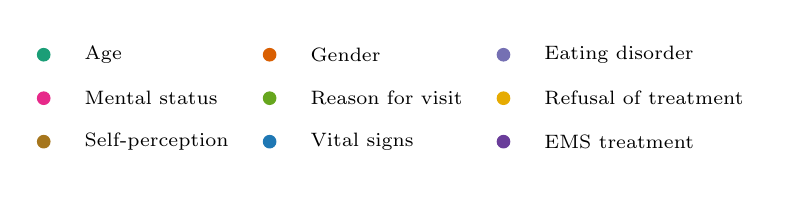
\begin{tikzpicture}
    \matrix[column sep=0.9em,row sep=0.35em,nodes={anchor=west,font=\scriptsize}] {
      \node[draw=HypFiveOne,fill=HypFiveOne,circle,inner sep=1.6pt] {}; & \node {Age}; & \node[draw=HypFiveTwo,fill=HypFiveTwo,circle,inner sep=1.6pt] {}; & \node {Gender}; & \node[draw=HypFiveThree,fill=HypFiveThree,circle,inner sep=1.6pt] {}; & \node {Eating disorder}; \\
      \node[draw=HypFiveFour,fill=HypFiveFour,circle,inner sep=1.6pt] {}; & \node {Mental status}; & \node[draw=HypFiveFive,fill=HypFiveFive,circle,inner sep=1.6pt] {}; & \node {Reason for visit}; & \node[draw=HypFiveSix,fill=HypFiveSix,circle,inner sep=1.6pt] {}; & \node {Refusal of treatment}; \\
      \node[draw=HypFiveSeven,fill=HypFiveSeven,circle,inner sep=1.6pt] {}; & \node {Self-perception}; & \node[draw=HypFiveEight,fill=HypFiveEight,circle,inner sep=1.6pt] {}; & \node {Vital signs}; & \node[draw=HypFiveNine,fill=HypFiveNine,circle,inner sep=1.6pt] {}; & \node {EMS treatment}; \\
    };
  \end{tikzpicture}

  \caption[Atomic and joint causal effects for the motivating MedQA example]{Atomic and interaction-aware causal effects for every concept in the motivating MedQA example. Points above the identity line receive a larger credited effect under FELICS; colors identify the concepts consistently across both panels.}
  \label{fig:hyp5-concept-identity}
\end{figure}

Figure~\ref{fig:hyp5-concept-identity} shows that the correction does not shift all concepts in a common direction. Note that the two panels deliberately use different axis scales because the GPT-OSS 120B effects are substantially smaller: its axes extend to $0.05$, whereas the Mistral Medium 3.5 axes extend to $0.45$. The largest positive shift occurs for refusal of treatment under Mistral Medium 3.5 ($\Delta\mathrm{CE}=0.070$), whereas self-perception has the largest negative shift ($\Delta\mathrm{CE}=-0.148$). Concepts assigned to singleton groups remain on the identity line by construction.

Table~\ref{tab:hyp5-faithfulness-comparison} additionally reports the posterior question-level faithfulness estimate $\mathcal{F}(\mathbf{x})$. For the two models evaluated in this work, the same Bayesian faithfulness pipeline and fixed EE vector were applied to the atomic and interaction-aware CE vectors, respectively, following Section~\ref{sec:controlled_atomic_baseline}. The posterior estimate increases by $0.131$ for GPT-OSS 120B and decreases by $0.033$ for Mistral Medium 3.5, while every 90\% credible interval contains zero. These results do not indicate a clear question-level faithfulness improvement, although the single-question setting necessarily produces substantial posterior uncertainty.

\begin{table}[htbp]
  \centering
  \caption[Question-level faithfulness for the motivating MedQA example]{Posterior question-level faithfulness for the motivating MedQA example. Published results from Matton et al.~\cite{mattonWalkTalkMeasuring2024} provide one singleton-intervention estimate per model; this work reports paired atomic and joint estimates. The intervals are 90\% credible intervals and $\Delta\mathcal{F}=\mathcal{F}_{\mathrm{joint}}-\mathcal{F}_{\mathrm{atomic}}$.}
  \label{tab:hyp5-faithfulness-comparison}
  \small
  \setlength{\tabcolsep}{4pt}
  \renewcommand{\arraystretch}{1.12}
  \pgfplotstabletypeset[
    col sep=comma,trim cells=true,
    columns={source,model,atomic_f,atomic_ci,joint_f,joint_ci,delta_f},
    columns/source/.style={column name={\textbf{Source}},string type,column type=l},
    columns/model/.style={column name={\textbf{Model}},string type,column type=l},
    columns/atomic_f/.style={column name={\textbf{$\mathcal{F}_{\mathrm{atomic}}$}},string type,column type=c},
    columns/atomic_ci/.style={column name={\textbf{90\% CI}},string type,column type=c},
    columns/joint_f/.style={column name={\textbf{$\mathcal{F}_{\mathrm{joint}}$}},string type,column type=c},
    columns/joint_ci/.style={column name={\textbf{90\% CI}},string type,column type=c},
    columns/delta_f/.style={column name={\textbf{$\Delta\mathcal{F}$}},string type,column type=c},
    every head row/.style={before row=\hline,after row=\hline},
    every last row/.style={after row=\hline},
    every even row/.style={before row={\rowcolor{gray!8}}},
  ]{data/rq5/faithfulness_comparison.csv}
\end{table}

In summary, FELICS increases the estimated effect of the eating-disorder concept but decreases the estimated effect of self-perception of weight for both evaluated models. The empirical result therefore does not satisfy the conjunctive hypothesis formulated for \rqref{rq:motivating_example}. It nevertheless demonstrates that joint interventions materially redistribute credited causal effect among the correlated concepts, rather than merely applying a uniform increase.
